\documentclass[11pt,a4paper]{article}
\usepackage[T1]{fontenc}
\usepackage[utf8]{inputenc}
\usepackage[spanish,es-noshorthands,es-tabla]{babel}
\usepackage{amsmath,amssymb,bm}
\usepackage{graphicx,booktabs,listings,geometry,enumitem,float}
\usepackage{siunitx,array}
\usepackage{hyperref}
\geometry{margin=2.4cm}
\graphicspath{{../../results/}}
\hypersetup{colorlinks=true,linkcolor=black,citecolor=blue,urlcolor=blue}
\lstset{basicstyle=\ttfamily\footnotesize,breaklines=true,columns=fullflexible,
  frame=single,framesep=3pt,showstringspaces=false}
\newcommand{\code}[1]{\texttt{#1}}
\newcommand{\tabla}[1]{\IfFileExists{../../results/comparison/tables/#1.tex}%
  {\input{../../results/comparison/tables/#1.tex}}%
  {\textit{Tabla pendiente: ejecute scripts/comparison/run\_all.py.}}}
\IfFileExists{../../results/comparison/tables/efficiency_macros.tex}%
  {% Generado por scripts/comparison/efficiency.py: cifras de tiempo del anexo y del paper.
\providecommand{\EffAlpha}{2.52}
\providecommand{\EffAlphaShort}{2.5}
\providecommand{\EffProdBeta}{0.96}
\providecommand{\EffTmmRecMin}{0.23}
\providecommand{\EffTmmRecMax}{0.33}
\providecommand{\EffTmmScalar}{44}
\providecommand{\EffTmmMaxM}{20}
\providecommand{\EffTmmMaxLayers}{10\,946}
\providecommand{\EffProdFirst}{0.5}
\providecommand{\EffProdLast}{291}
\providecommand{\EffPweFirstM}{2}
\providecommand{\EffPweFirst}{3.3~ms}
\providecommand{\EffPweLastM}{10}
\providecommand{\EffPweLast}{32.5~s}
\providecommand{\EffPweGrowth}{3.4}
\providecommand{\EffExtrapAM}{12}
\providecommand{\EffExtrapA}{6~min}
\providecommand{\EffExtrapBM}{15}
\providecommand{\EffExtrapB}{3.7~h}
\providecommand{\EffExtrapBMem}{16~GB}
\providecommand{\EffMemEight}{19~MB}
\providecommand{\EffWpM}{5}
\providecommand{\EffWpTmmErr}{3\times10^{-15}}
\providecommand{\EffWpTmmMin}{1.4}
\providecommand{\EffWpTmmMax}{31}
\providecommand{\EffWpErrExp}{3.1}
\providecommand{\EffWpTimeExp}{2.5}
\providecommand{\EffWpTradeExp}{1.3}
\providecommand{\EffWpBestErr}{1\times10^{-6}}
\providecommand{\EffWpBestN}{385}
\providecommand{\EffWpBestTime}{1.2~s}
\providecommand{\EffWpSpeedRatio}{4\times10^{4}}
\providecommand{\EffWpErrRatio}{4\times10^{8}}
\providecommand{\EffWpTargetN}{3\times10^{4}}
\providecommand{\EffWpTargetMem}{68~GB}
\providecommand{\EffWpTargetTime}{23~h}
\providecommand{\EffFigTmmTotal}{0.32~s}
\providecommand{\EffFigPweTotal}{5.3~h}
\providecommand{\EffFigRatioMin}{2\times10^{4}}
\providecommand{\EffFigRatioMax}{4\times10^{5}}
\providecommand{\EffFigWallMin}{45}
\providecommand{\EffFigWallMax}{319}
\providecommand{\EffFigTmmMin}{2.9}
\providecommand{\EffFigTmmMax}{3.4}
\providecommand{\EffBookN}{101}
\providecommand{\EffBookPwe}{116~ms}
\providecommand{\EffBookTmm}{78~ms}
\providecommand{\EffBookGrid}{14~ms}
\providecommand{\EffBookGridPoints}{60\,001}
\providecommand{\EffBookErr}{5\times10^{-6}}
}{}

\title{Anexo: comparación de resultados\\
matriz de transferencia (TMM) frente a ondas planas (PWE)}
\author{Emanuel Orozco Gallego}
\date{28 de septiembre de 2026}

\begin{document}
\maketitle

\begin{abstract}
Este anexo compara, figura por figura, los resultados del PRB 81, 153101 (2010)
calculados con dos métodos independientes: la matriz de transferencia (TMM),
que es exacta para medios estratificados, y la expansión en ondas planas (PWE)
en la forma $k(\omega)$ con la regla inversa de Li, descrita en el documento
\textit{El método de expansión en ondas planas para superredes de Fibonacci}.
Para cada figura se muestran las curvas superpuestas, el error punto a punto de
la semitraza $R_m$, el número de subbandas y, en las Figs.~5--6, el error de
cada borde de banda. Además, se mide el tiempo de cómputo de los dos métodos en
un núcleo (escalamiento con el orden de Fibonacci, trabajo-precisión, costo por
figura y memoria) y se concluye cuál es el más adecuado y por qué: la TMM, que es
exacta y entre $\EffFigRatioMin$ y $\EffFigRatioMax$ veces más rápida por figura.
Todas las cifras y tablas se generan desde los datos con
\code{scripts/comparison/run\_all.py}.
\end{abstract}

\tableofcontents

%=====================================================================
\section{Qué se compara y cómo}
%=====================================================================

\paragraph{Cantidad común.} Ambos métodos entregan la semitraza
$R_m(\nu,\theta)=\cos(kL_m)$ de la celda $S_m$:
\begin{itemize}
\item TMM: $R_m=\tfrac12\operatorname{Tr}(M_{F_m}\cdots M_1)$, producto de las
matrices $2\times2$ de cada capa;
\item PWE: $R_m=\mathrm{Re}\cos\tilde k$, con $\tilde k=kL_m$ el autovalor de
Bloch de menor $|\mathrm{Im}\,\tilde k|$ del problema cuadrático
$\tilde k^2P+\tilde k(PG+GP)+(GPG-F)=0$ con $N=2hF_m+1$ ondas planas.
\end{itemize}
Las dos funciones se evalúan exactamente en la misma malla de frecuencias.

\paragraph{Métricas.}
\begin{enumerate}[label=(\alph*)]
\item $\max|\Delta R|=\max|R_{\rm PWE}-R_{\rm TMM}|$ en las frecuencias que la
TMM clasifica como banda ($|R|\le1$); en los gaps se usa el error relativo
$|\Delta R|/|R_{\rm TMM}|$ porque $|R|$ crece exponencialmente.
\item Acuerdo banda/gap: fracción de frecuencias con la misma clasificación.
\item Conteo de subbandas de plasmón-polaritón frente a la regla $F_{m-2}$.
\item Bordes de subbanda (Figs.~5--6): ambos métodos pasan por el \emph{mismo}
localizador (malla logarítmica en $\nu_m-\nu$, detección de cambios de signo y
refinamiento de Brent); se comparan los bordes y el ancho $w$ de cada subbanda.
\item Tiempo de cómputo, medido en un núcleo para los dos métodos
(Sec.~\ref{sec:tiempo}), y a partir de él, cuál método conviene y por qué.
\end{enumerate}

\paragraph{Parámetros.} Física en \code{configs/figure\_0N.yaml} (idéntica para
los dos métodos) y numérica del PWE en \code{configs/pwe/figure\_0N.yaml}:
$h=8$ armónicos por capa en las Figs.~1--3, $h=16$ en la Fig.~4, $h=16$ para
$m\le4$ y $h=8$ para $m=5,6$ en las Figs.~5--6.

%=====================================================================
\section{Resumen de resultados}
%=====================================================================

\begin{itemize}
\item \textbf{Relación de dispersión (Figs.~1--4).} Las curvas del PWE caen sobre
las de la TMM. El error en las bandas es de $10^{-7}$--$10^{-5}$ en casi todo el
rango, con picos locales en los polos de Drude ($\mu_B=0$ o $\varepsilon_B=0$).
Crece al bajar la frecuencia porque el contraste entre capas aumenta: a
0.15~GHz, $\varepsilon_B=1-\nu_e^2/\nu^2\approx-399$ y, en la Fig.~1,
también $\mu_B\approx-399$. Con 8 armónicos por capa el error máximo es
$\sim\!2\times10^{-2}$ en la Fig.~1 (con $\mu_B$, que es la función dentro de la
derivada en TE, a $-399$) y $4.5\times10^{-4}$ en la Fig.~3 ($\mu_B\approx-43$). La
clasificación banda/gap coincide en más del 99.9\% de las frecuencias; las
discrepancias son frecuencias sueltas pegadas a un borde de banda.
\item \textbf{Conteo de subbandas.} TMM, PWE y la regla $F_{m-2}$ coinciden en
todos los casos (Tabla~\ref{tab:conteos}, Tabla~\ref{tab:fig5}, Tabla~\ref{tab:fig6}).
\item \textbf{Bordes (Figs.~5--6).} Errores relativos de ancho entre $10^{-9}$ y
$4\times10^{-6}$ y errores de borde menores que $10^{-7}$~GHz: el PWE confirma la posición y el ancho de cada subbanda.
\item \textbf{Tiempo y método recomendado.} En un núcleo, las seis figuras cuestan
\EffFigTmmTotal{} con la TMM y unas \EffFigPweTotal{} con el PWE, entre
$\EffFigRatioMin$ y $\EffFigRatioMax$ veces más por figura. El costo del PWE crece
como $N^{\EffAlphaShort}$ con $N\propto F_m$, mientras que el de la TMM casi no
depende de $m$. Para la misma precisión, la TMM llega al redondeo de la máquina en
microsegundos y el PWE necesita \EffWpBestTime{} por frecuencia para un error de
$\EffWpBestErr$. La TMM es el método óptimo para este problema y el PWE queda
como verificación independiente y como base para 2D (Sec.~\ref{sec:tiempo}).
\item \textbf{Límite del PWE.} A menos de $\sim\!10^{-6}$~GHz de $\nu_m$ (gaps con
$|R|\gtrsim10^4$) el PWE produce bandas espurias, que la validación con
$1.5N$ ondas planas descarta de forma automática.
\end{itemize}

%=====================================================================
\section{Figuras 1--4: relación de dispersión}
%=====================================================================

En las superposiciones, la línea es la TMM y los círculos huecos negros el PWE
(una muestra de cada varias para no tapar la línea). Las figuras de error muestran
$|R_{\rm PWE}-R_{\rm TMM}|/\max(1,|R_{\rm TMM}|)$; las franjas grises son los gaps
de la TMM.

\begin{table}[H]
\centering
\caption{Acuerdo por barrido: error máximo en bandas, acuerdo banda/gap y tiempo
de cada barrido. La TMM corre en un proceso; el tiempo del PWE es de pared con 16
procesos en paralelo (el costo en un núcleo está en la Tabla~\ref{tab:tiempo-figuras}).}
\label{tab:dispersion}
\resizebox{\linewidth}{!}{\tabla{dispersion}}
\end{table}

\subsection{Figura 1 ($\nu_e=\nu_m=3$ GHz)}

\begin{figure}[H]
\centering
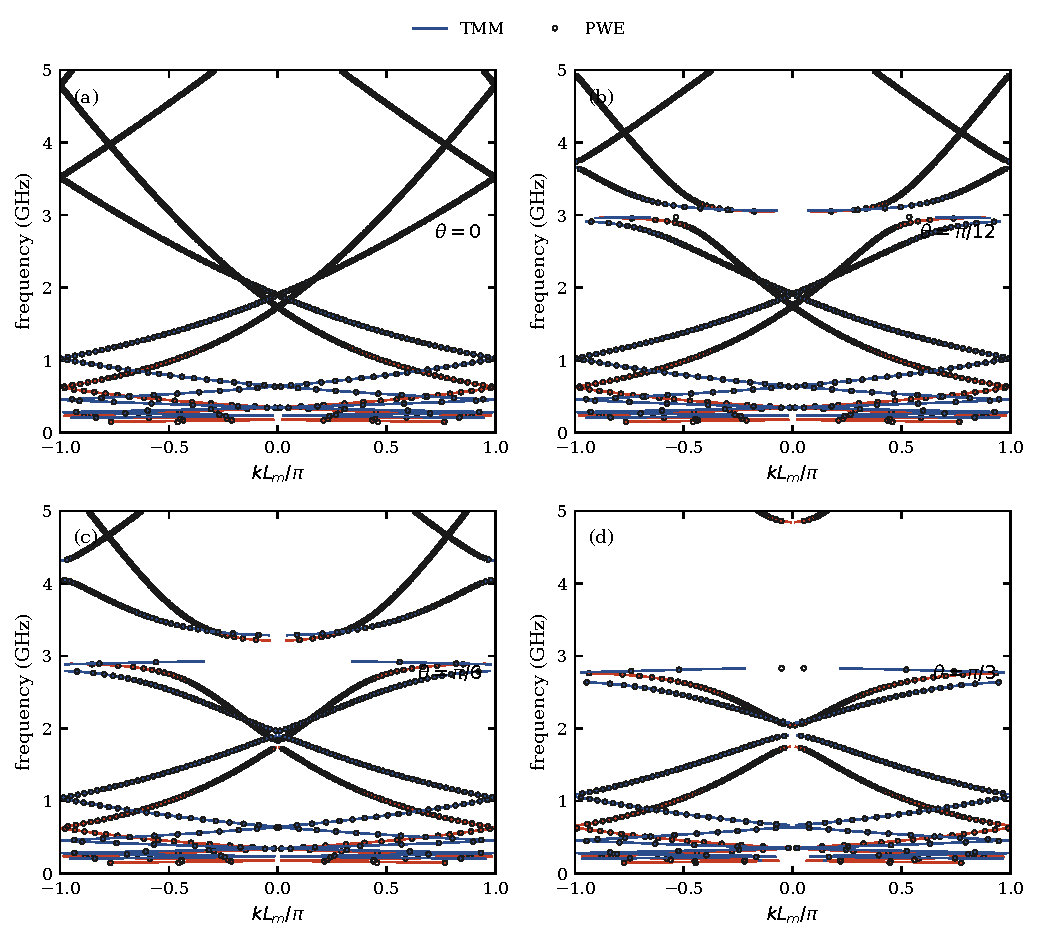
\includegraphics[width=0.88\linewidth]{comparison/figure_01/output/figure_01_overlay.pdf}
\caption{Fig.~1: relación de dispersión TMM (líneas) y PWE (círculos) para $m=3,4$
y cuatro ángulos.}
\end{figure}

\begin{figure}[H]
\centering
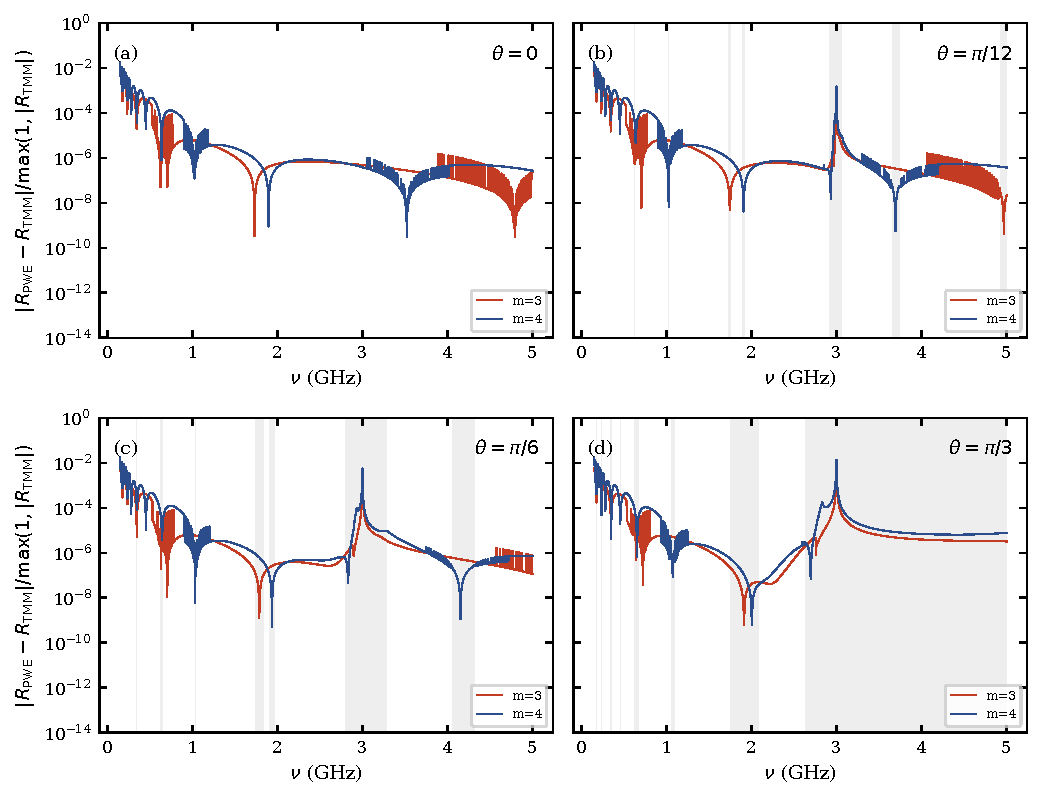
\includegraphics[width=0.88\linewidth]{comparison/figure_01/output/figure_01_error.pdf}
\caption{Fig.~1: error de la semitraza del PWE respecto a la TMM.}
\end{figure}

\subsection{Figura 2 (vecindad de $\nu_m=3$ GHz, $\theta=\pi/3$)}

\begin{figure}[H]
\centering
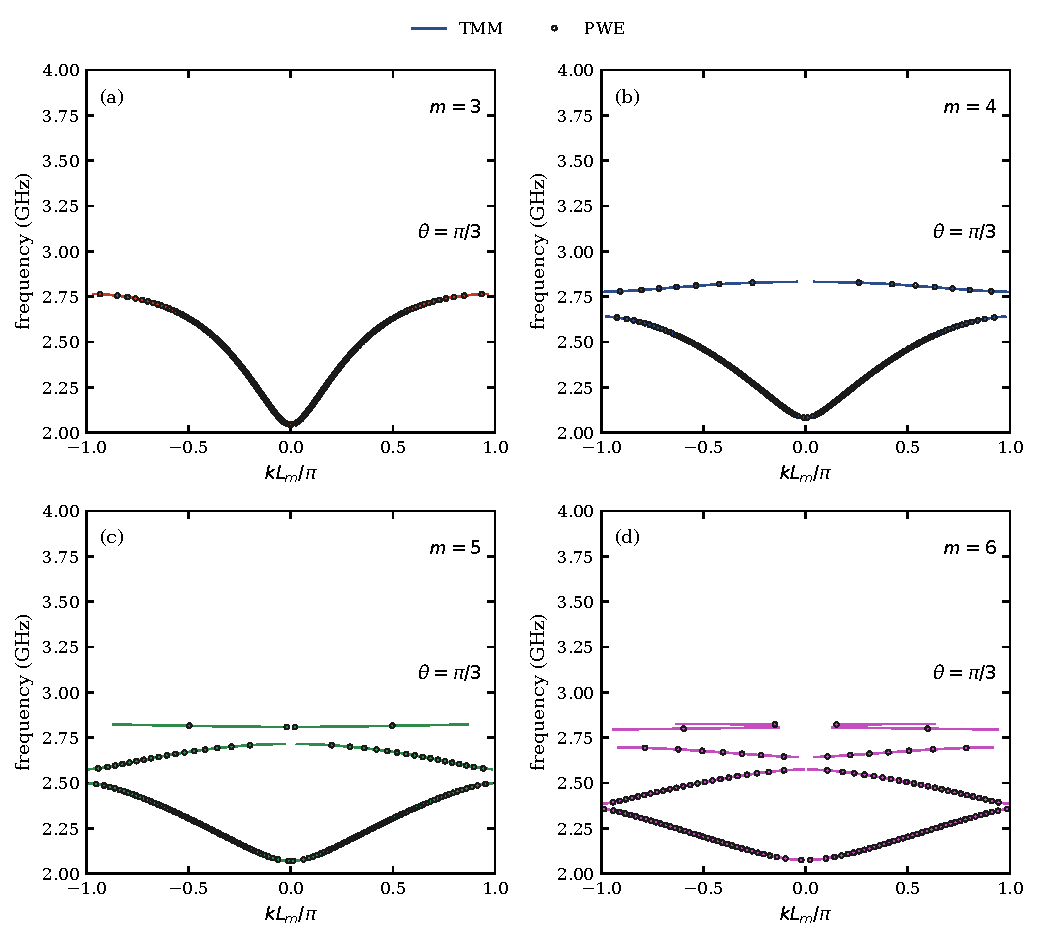
\includegraphics[width=0.88\linewidth]{comparison/figure_02/output/figure_02_overlay.pdf}
\caption{Fig.~2: subbandas de plasmón-polaritón para $m=3\dots6$; el PWE
reproduce las $F_{m-2}=1,2,3,5$ subbandas.}
\end{figure}

\begin{figure}[H]
\centering
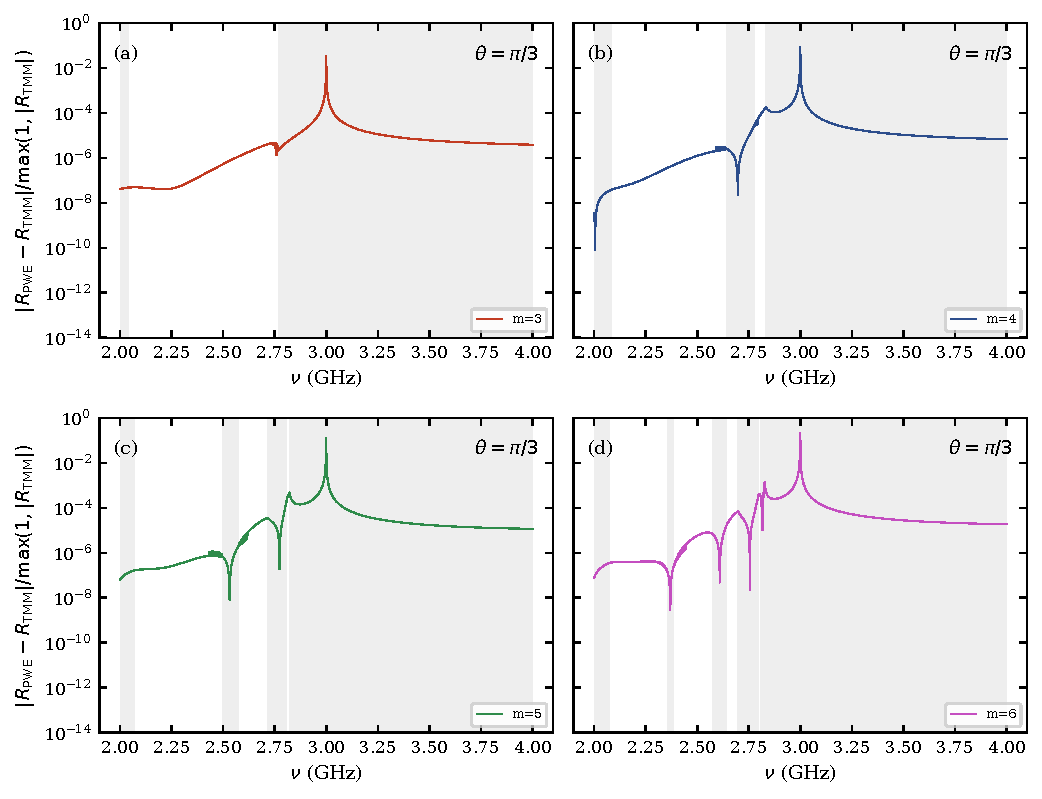
\includegraphics[width=0.88\linewidth]{comparison/figure_02/output/figure_02_error.pdf}
\caption{Fig.~2: error de la semitraza.}
\end{figure}

\subsection{Figura 3 ($\nu_e=3$ GHz, $\nu_m=1$ GHz)}

\begin{figure}[H]
\centering
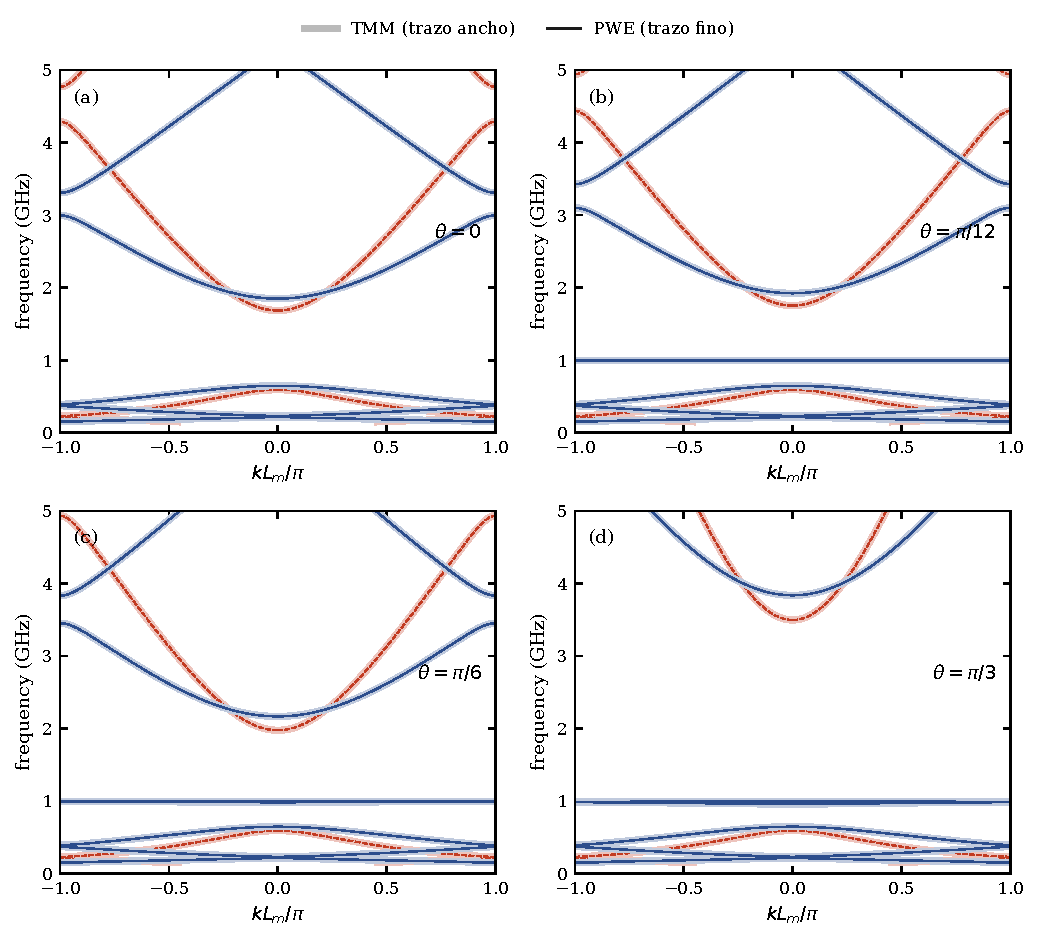
\includegraphics[width=0.88\linewidth]{comparison/figure_03/output/figure_03_overlay.pdf}
\caption{Fig.~3: relación de dispersión TMM y PWE. La banda plana en 1~GHz es el
plasmón-polaritón magnético dentro del gap $\langle n\rangle=0$.}
\end{figure}

\begin{figure}[H]
\centering
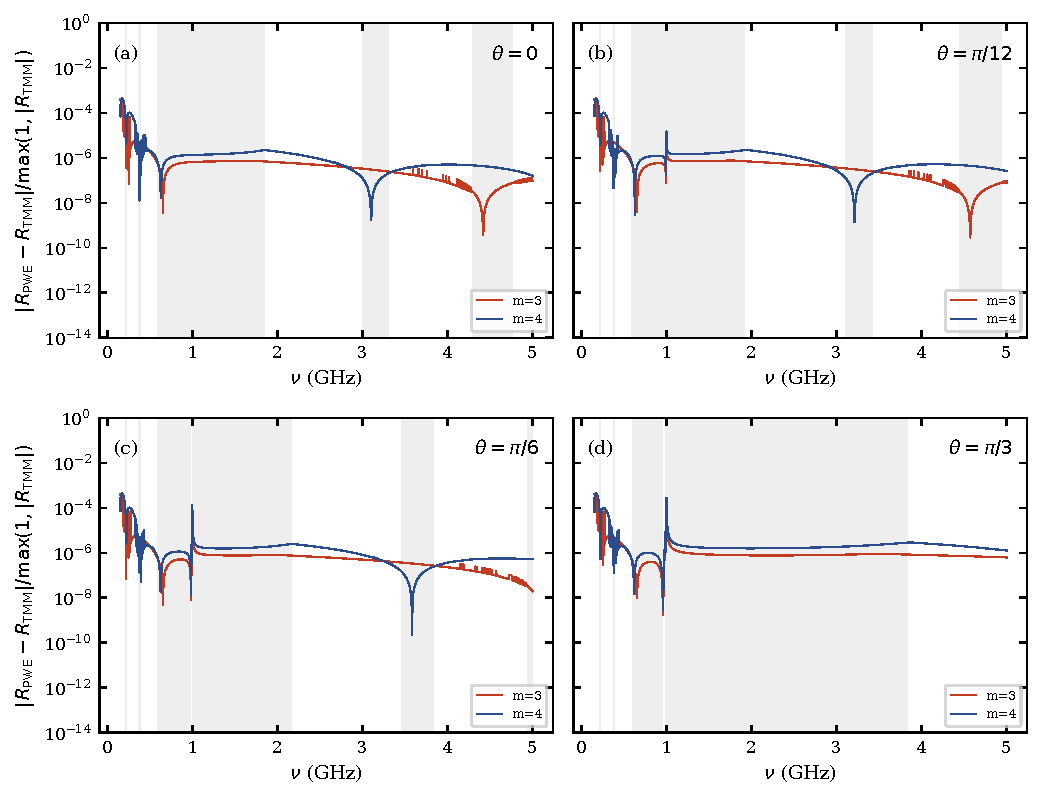
\includegraphics[width=0.88\linewidth]{comparison/figure_03/output/figure_03_error.pdf}
\caption{Fig.~3: error de la semitraza. El pico en 1~GHz es el polo de
$1/\mu_B$; el aumento por debajo de 0.5~GHz se debe al gran contraste
$|\varepsilon_B|\gg1$.}
\end{figure}

\subsection{Figura 4 (ampliación de los polaritones de la Fig.~3)}

\begin{figure}[H]
\centering
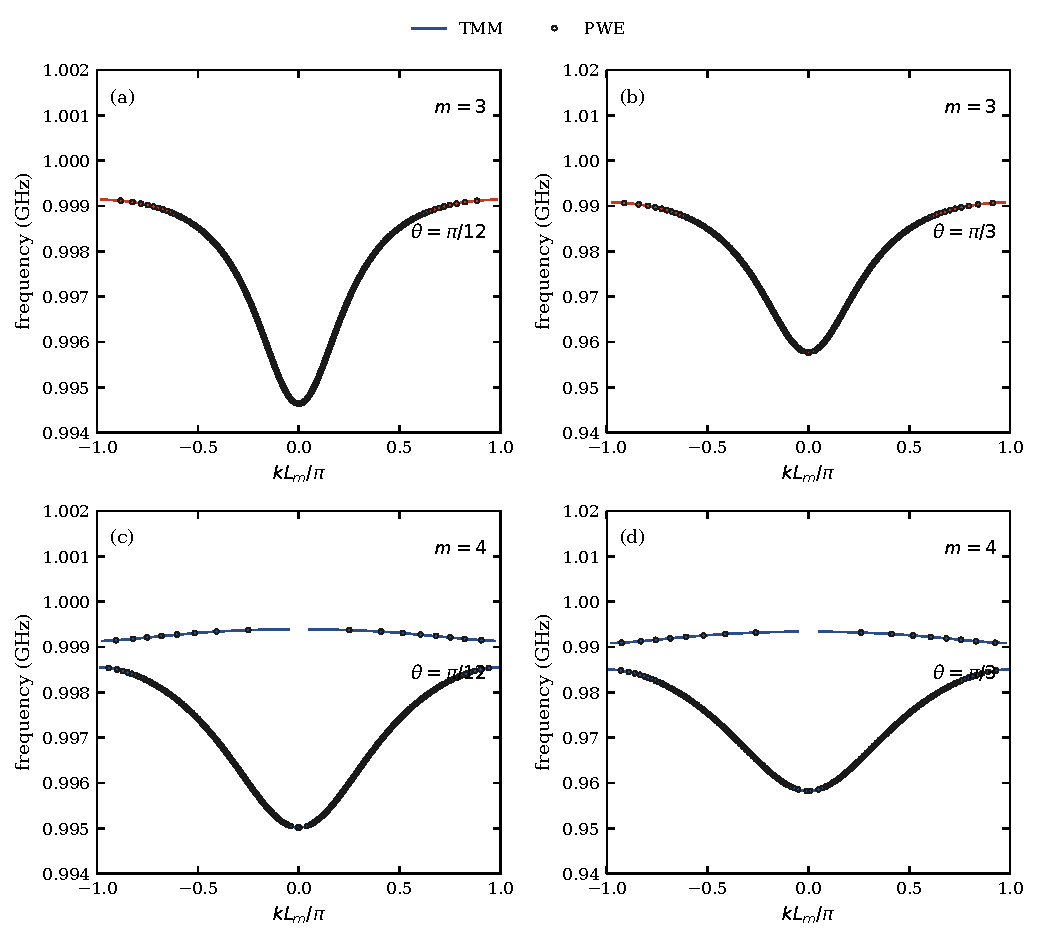
\includegraphics[width=0.88\linewidth]{comparison/figure_04/output/figure_04_overlay.pdf}
\caption{Fig.~4: una subbanda para $m=3$ y dos para $m=4$, con los dos métodos.}
\end{figure}

\begin{figure}[H]
\centering
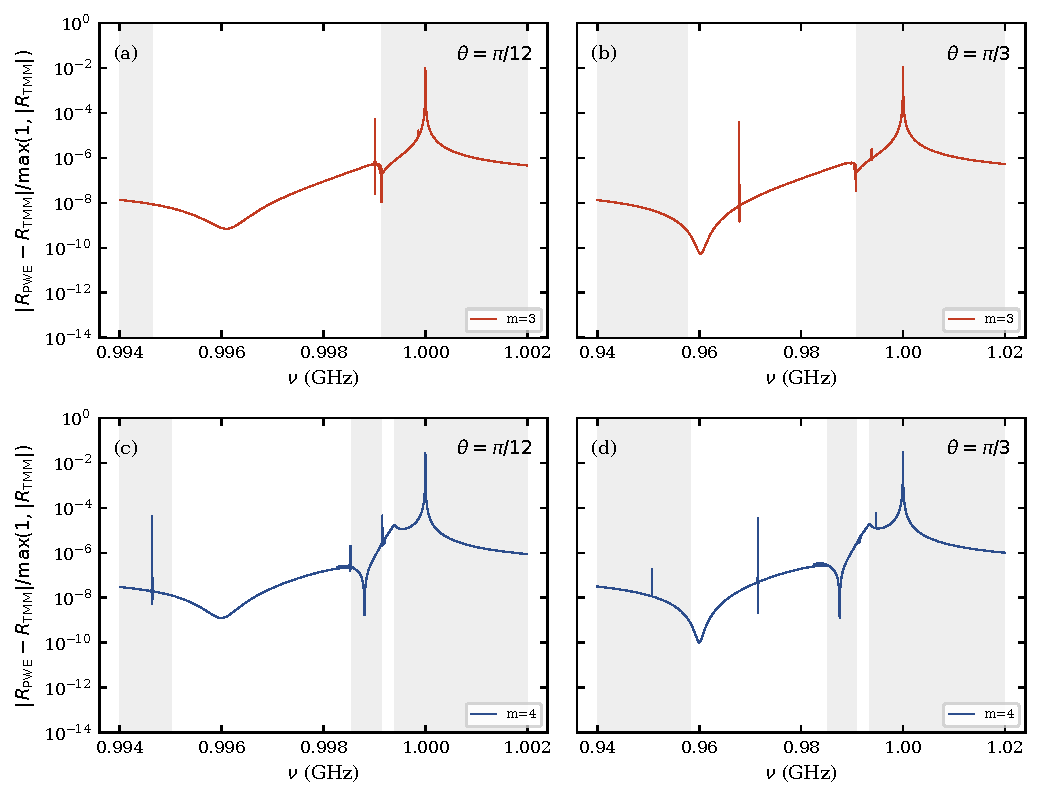
\includegraphics[width=0.88\linewidth]{comparison/figure_04/output/figure_04_error.pdf}
\caption{Fig.~4: error de la semitraza en las ventanas ampliadas.}
\end{figure}

\begin{table}[H]
\centering
\caption{Número de subbandas detectadas en las Figs.~2 y 4.}
\label{tab:conteos}
\tabla{mode_counts}
\end{table}

%=====================================================================
\section{Figuras 5--6: bordes y anchos de las subbandas}
%=====================================================================

Aquí la comparación es más exigente: las subbandas miden entre $10^{-8}$ y
$10^{-3}$~GHz y están a menos de $10^{-2}$~GHz de $\nu_m=1$~GHz. Para cada caso se
buscan las subbandas con los dos métodos en la misma malla y se emparejan.
Las bandas del PWE que no pasan la validación con $1.5N$ ondas planas se
registran como rechazadas en \code{results/pwe/figure\_0N/data/summary.json}.

\begin{figure}[H]
\centering
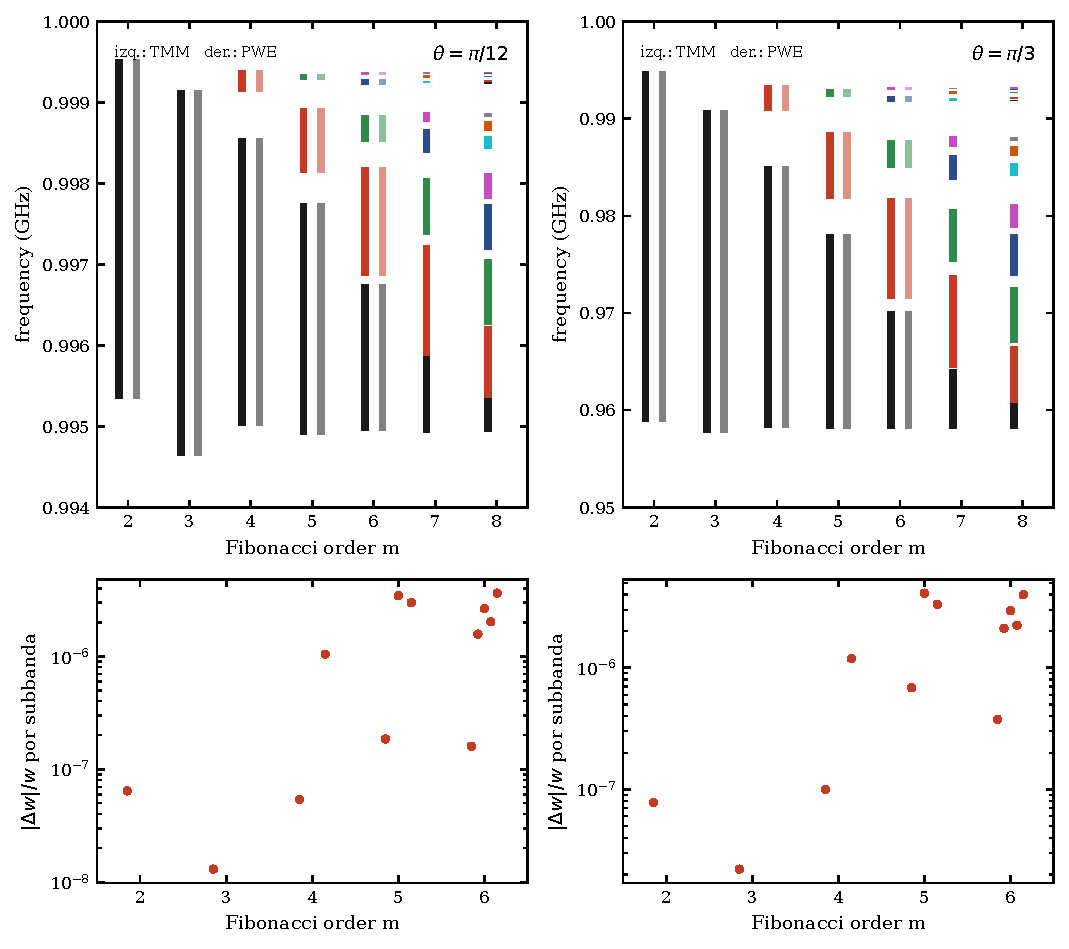
\includegraphics[width=\linewidth]{comparison/figure_05/output/figure_05_comparison.pdf}
\caption{Fig.~5. Arriba: intervalos permitidos debajo de $\nu_m$ para cada orden
$m$; en cada orden, la barra izquierda es la TMM y la derecha (más clara) el PWE.
Los órdenes $m=7,8$ solo se calculan con la TMM. Abajo: error relativo del ancho
de cada subbanda del PWE respecto a la TMM.}
\end{figure}

\begin{table}[H]
\centering
\caption{Fig.~5: conteo y errores de borde y de ancho por caso.}
\label{tab:fig5}
\resizebox{\linewidth}{!}{\tabla{figure_05}}
\end{table}

\begin{figure}[H]
\centering
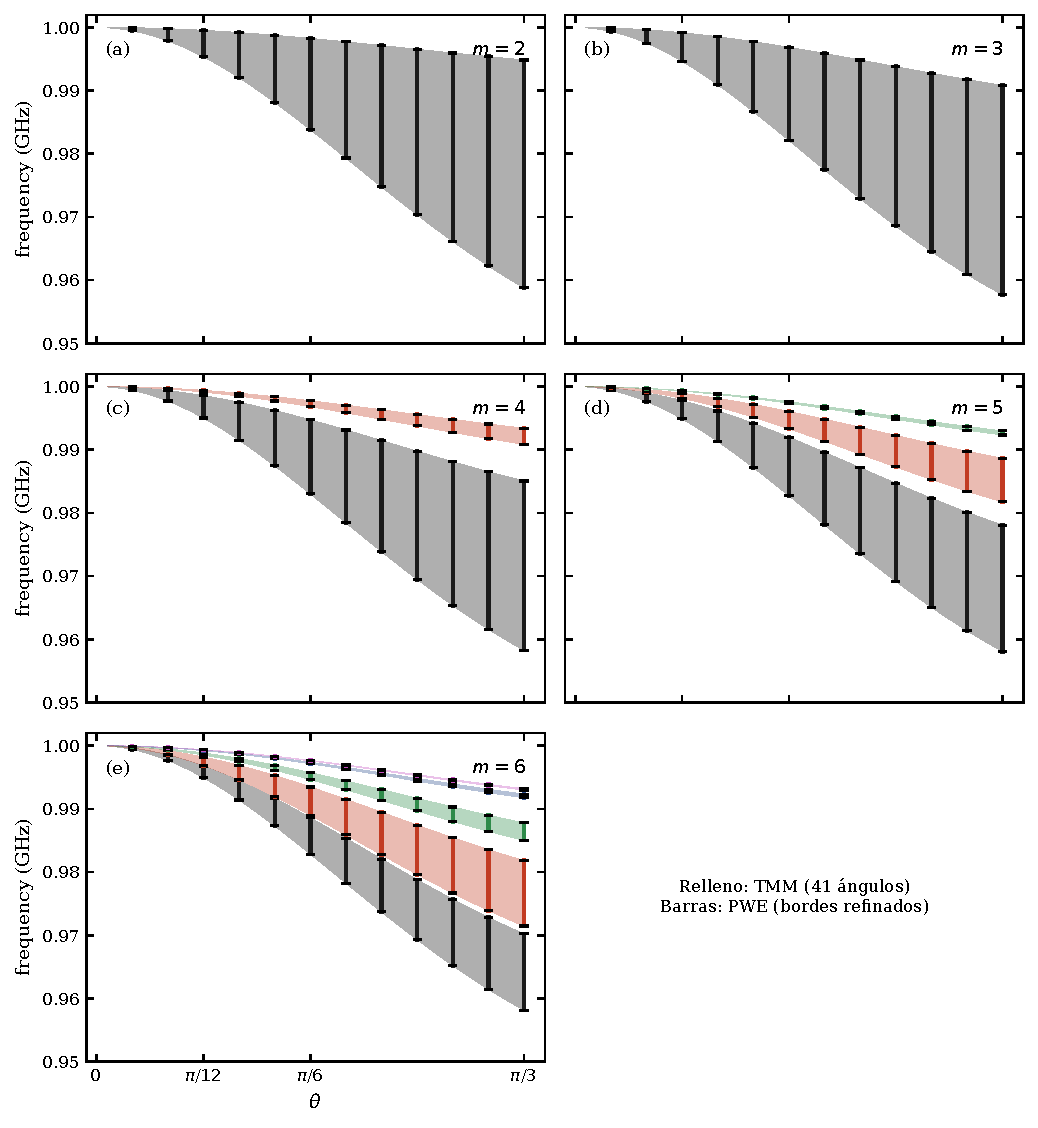
\includegraphics[width=\linewidth]{comparison/figure_06/output/figure_06_overlay.pdf}
\caption{Fig.~6: subbandas frente al ángulo de incidencia. Relleno: TMM
(41 ángulos); barras: subbandas del PWE con bordes refinados (12 ángulos,
$\theta=5^\circ\dots60^\circ$). Cada color es una subbanda.}
\end{figure}

\begin{figure}[H]
\centering
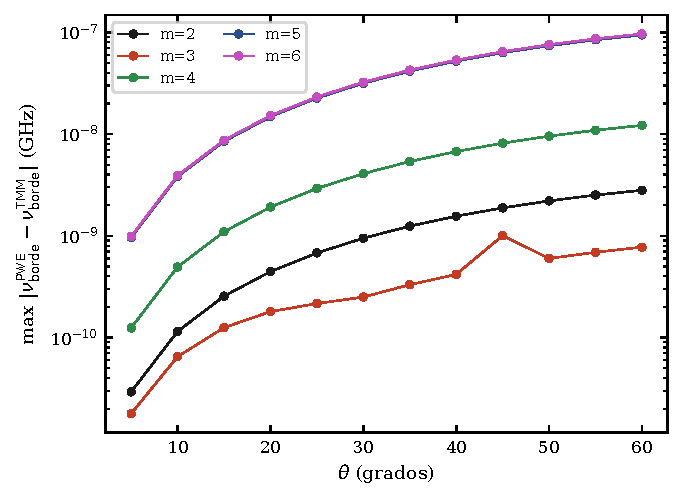
\includegraphics[width=0.85\linewidth]{comparison/figure_06/output/figure_06_edge_error.pdf}
\caption{Fig.~6: error máximo de los bordes de las subbandas del PWE respecto a
la TMM (en GHz), por orden y ángulo. El error absoluto crece con el ángulo a la
par que el ancho de las subbandas (el error relativo del ancho se mantiene por
debajo de $5\times10^{-6}$) y es mayor para $m=5,6$, donde se usan 8 armónicos por
capa en lugar de 16.}
\end{figure}

\begin{table}[H]
\centering
\caption{Fig.~6: resumen por orden de Fibonacci.}
\label{tab:fig6}
\tabla{figure_06}
\end{table}

%=====================================================================
\section{Estudios numéricos}
%=====================================================================

\subsection{Convergencia}

\begin{figure}[H]
\centering
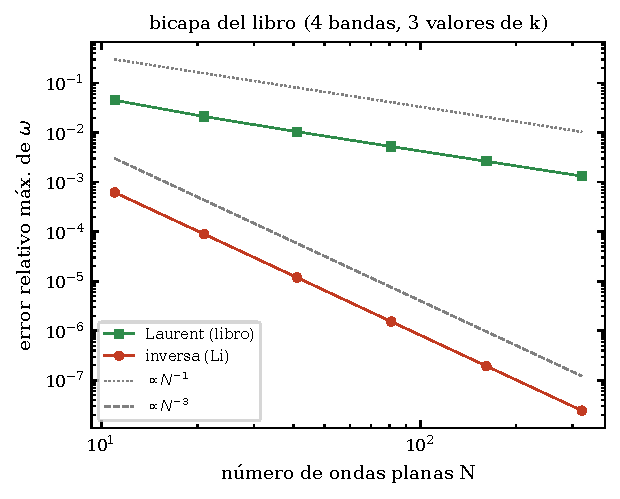
\includegraphics[width=0.49\linewidth]{pwe/convergence/output/book_convergence.pdf}\hfill
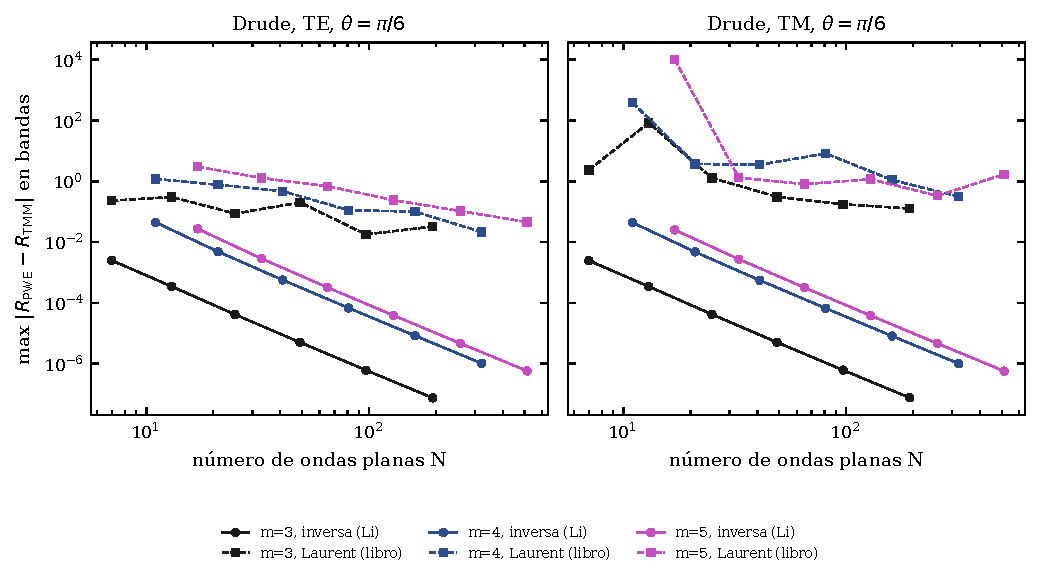
\includegraphics[width=0.49\linewidth]{pwe/convergence/output/drude_convergence.pdf}
\caption{Izquierda: cristal del libro, error de las bandas frente a $N$.
Derecha: superred de Drude ($m=3,4,5$, $\theta=\pi/6$), error en $R$ frente a la TMM en TE y TM.
La regla inversa converge varios órdenes por delante de la de Laurent.}
\end{figure}

\begin{table}[H]
\centering
\caption{Cristal del libro: error relativo máximo de las cuatro primeras bandas
en $ka/\pi=0.25,\,0.5,\,0.75$.}
\tabla{book_convergence}
\end{table}

\subsection{Costo y precisión}

\begin{table}[H]
\centering
\caption{Costo por frecuencia y precisión según el orden de Fibonacci.}
\label{tab:costo}
\resizebox{\linewidth}{!}{\tabla{cost}}
\end{table}

\begin{figure}[H]
\centering
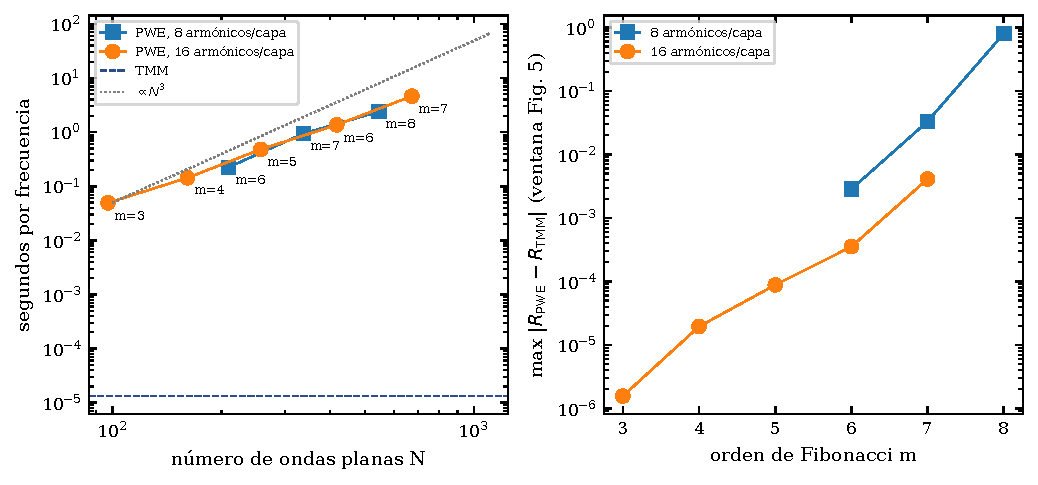
\includegraphics[width=0.6\linewidth]{pwe/convergence/output/cost_and_accuracy.pdf}
\caption{Tiempo por frecuencia y error máximo del PWE según $m$ y el número de
armónicos por capa. El análisis de tiempos completo está en la Sec.~\ref{sec:tiempo}.}
\end{figure}

\subsection{Límite de validez del PWE cerca de $\nu_m$}

\begin{figure}[H]
\centering
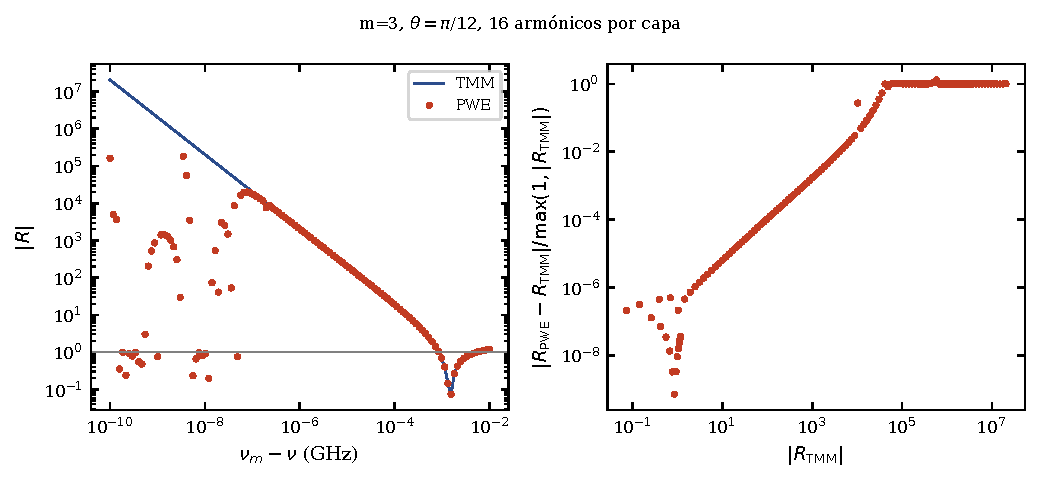
\includegraphics[width=0.8\linewidth]{pwe/convergence/output/validity_near_nu_m.pdf}
\caption{Semitraza junto a $\nu_m$: TMM y PWE con varios $N$. Donde
$|R|\gtrsim10^4$ el PWE se separa de la TMM y depende de $N$; de ahí la
validación de bandas con $1.5N$ ondas planas.}
\end{figure}

\subsection{Forma $\omega(k)$: contaminación espectral}
\label{sec:contaminacion}

\begin{figure}[H]
\centering
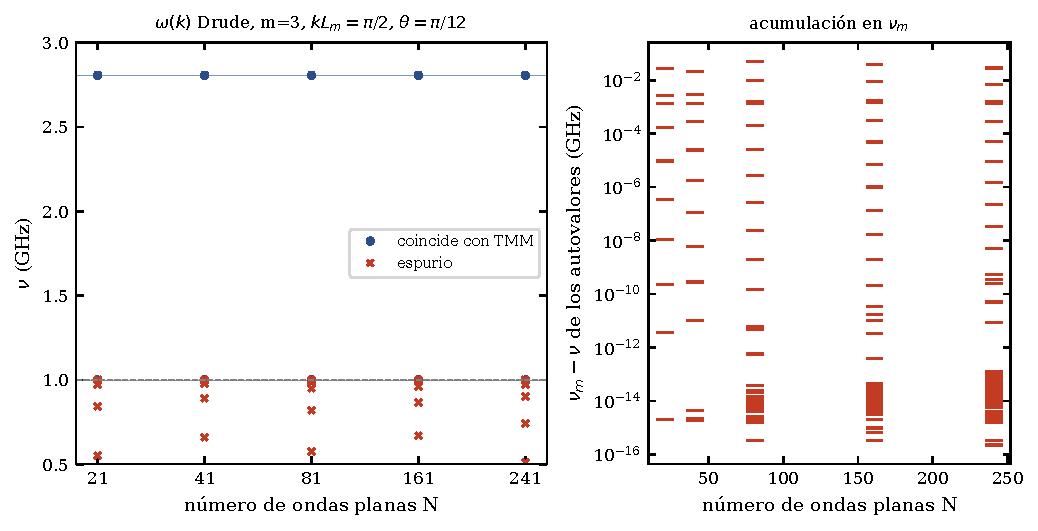
\includegraphics[width=\linewidth]{pwe/spectral_pollution/output/spectral_pollution.pdf}
\caption{Forma $\omega(k)$ del libro aplicada a Drude ($m=3$, $kL_m=\pi/2$,
$\theta=\pi/12$): solo dos autovalores coinciden con la TMM; el resto son
espurios y se acumulan en $\nu_m$.}
\end{figure}

\begin{table}[H]
\centering
\caption{Autovalores del problema $\omega(k)$ en 0.5--3~GHz y espurios.}
\tabla{pollution}
\end{table}

%=====================================================================
\section{Tiempo de cómputo y elección del método}
\label{sec:tiempo}
%=====================================================================

Esta sección responde dos preguntas: cuánto tarda cada método en producir los
mismos resultados y cuál de los dos conviene para este problema. Todas las
mediciones se hicieron en el mismo equipo, en \emph{un} núcleo y con un solo hilo
de BLAS, con \code{scripts/comparison/efficiency.py}
(configuración en \code{configs/comparison/efficiency.yaml}). Así los tiempos de
los dos métodos se pueden comparar directamente. Los tiempos de pared con 16
procesos que aparecen en la Tabla~\ref{tab:dispersion} solo se citan como
referencia.

\subsection{De dónde sale la diferencia de costo}

\paragraph{TMM.} Una evaluación de $R_m(\nu)$ es el producto de $F_m$ matrices
$2\times2$, cada una con la solución \emph{exacta} de la ecuación de onda dentro de
una capa homogénea. El costo es $O(F_m)$. Con la recurrencia de semitrazas
$R_m=2R_{m-1}R_{m-2}-R_{m-3}$ basta calcular $R_0$, $R_1$, $R_2$ y hacer $m$
multiplicaciones, es decir, $O(m)$. La memoria es la de una matriz $2\times2$, y el
único error es el de redondeo.

\paragraph{PWE.} Cada frecuencia requiere armar las matrices de Toeplitz
$N\times N$, invertir $[\![\chi]\!]$ y calcular los $2N$ autovalores de la matriz
compañera $2N\times2N$. Ambas operaciones cuestan $O(N^3)$. Como
$N=2hF_m+1$ crece como $F_m\propto\varphi^m$ ($\varphi$ es la razón áurea), el
costo crece como $\varphi^{3m}\approx4.2^m$ y la memoria como
$64N^2$~bytes. Además, el truncamiento de la serie de Fourier de un perfil
discontinuo deja un error que solo baja algebraicamente con $N$.

\begin{figure}[H]
\centering
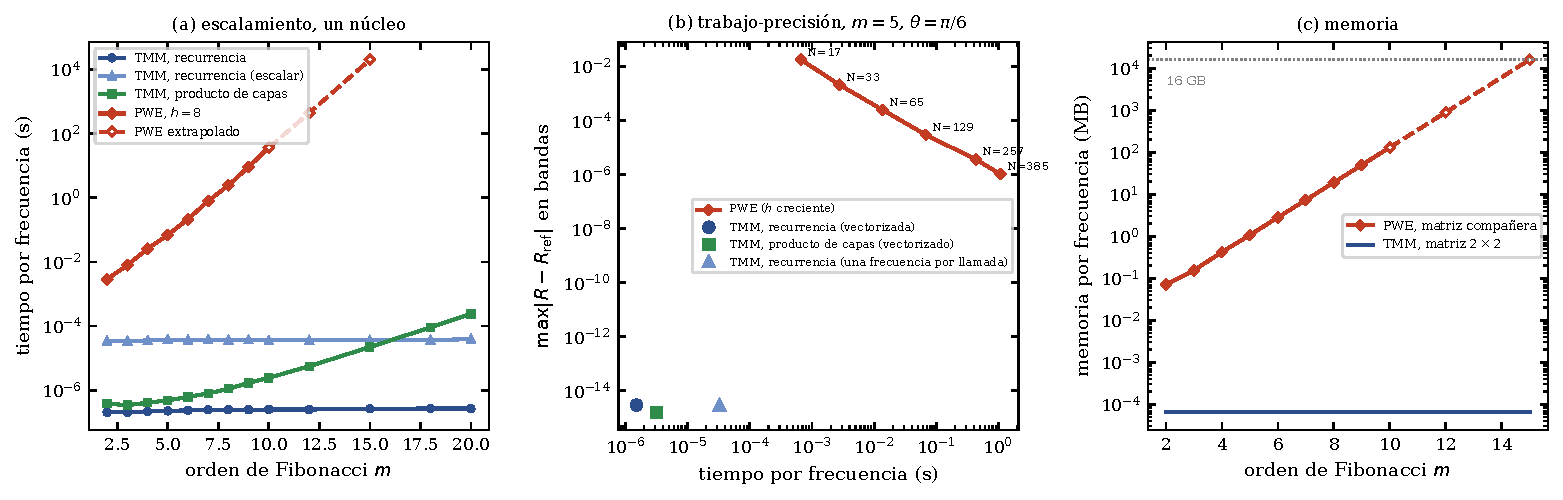
\includegraphics[width=\linewidth]{comparison/efficiency/output/efficiency.pdf}
\caption{Eficiencia en un núcleo. (a) Tiempo por frecuencia frente al orden de
Fibonacci en la ventana de la Fig.~5 ($\theta=\pi/12$): TMM por recurrencia
(vectorizada sobre 1000 frecuencias y llamada frecuencia por frecuencia), TMM por
producto de capas y PWE con $h=8$ armónicos por capa. Los puntos huecos son
extrapolaciones del ajuste $t\propto N^{\EffAlpha}$. (b) Diagrama trabajo-precisión
para $m=5$, $\theta=\pi/6$, 40 frecuencias entre 0.3 y 5~GHz: error máximo de
$R$ en las bandas frente a una referencia TMM en precisión extendida, contra el
tiempo por frecuencia. (c) Memoria por frecuencia: la matriz compañera del PWE
frente a la matriz $2\times2$ de la TMM.}
\label{fig:eficiencia}
\end{figure}

\subsection{Escalamiento con el orden de Fibonacci}

La Tabla~\ref{tab:escalamiento} y la Fig.~\ref{fig:eficiencia}(a) confirman el
análisis:
\begin{itemize}
\item La TMM por recurrencia tarda entre \EffTmmRecMin{} y \EffTmmRecMax~$\mu$s por
frecuencia desde $m=2$ hasta $m=\EffTmmMaxM$ (\EffTmmMaxLayers{} capas); su costo
prácticamente no depende de $m$. Llamada frecuencia por frecuencia tarda unos
\EffTmmScalar~$\mu$s, casi todo sobrecarga del intérprete de Python.
\item La TMM por producto de capas crece como $F_m^{\EffProdBeta}$, es decir,
linealmente con el número de capas, como se esperaba (\EffProdFirst~$\mu$s con
$m=2$ y \EffProdLast~$\mu$s con $m=\EffTmmMaxM$).
\item El PWE crece como $N^{\EffAlpha}$: pasa de \EffPweFirst{} ($m=\EffPweFirstM$)
a \EffPweLast{} ($m=\EffPweLastM$), y cada orden adicional multiplica el tiempo por
$\approx\EffPweGrowth$. El exponente es menor que 3 porque con estos tamaños el
álgebra lineal aún no está en su régimen asintótico. Al extrapolar,
$m=\EffExtrapAM$ tardaría unos \EffExtrapA{} y $m=\EffExtrapBM$ unas \EffExtrapB{}
\emph{por frecuencia}, con \EffExtrapBMem{} solo para la matriz compañera.
\end{itemize}

\begin{table}[H]
\centering
\caption{Tiempo por frecuencia en un núcleo según el orden de Fibonacci
($h=8$ armónicos por capa en el PWE). PWE/TMM se calcula con la TMM llamada
frecuencia por frecuencia, que es el caso más desfavorable para la TMM.
$^*$Extrapolado con $t\propto N^{\EffAlpha}$; la memoria es la de la matriz compañera.}
\label{tab:escalamiento}
\resizebox{\linewidth}{!}{\tabla{efficiency_scaling}}
\end{table}

\subsection{Tiempo necesario para una precisión dada}

El diagrama trabajo-precisión (Fig.~\ref{fig:eficiencia}(b),
Tabla~\ref{tab:trabajo-precision}) compara lo que cada método entrega por unidad
de tiempo. La TMM llega al redondeo de la máquina ($\sim\!\EffWpTmmErr$) en
\EffWpTmmMin--\EffWpTmmMax~$\mu$s por frecuencia. El error del PWE baja como
$N^{-\EffWpErrExp}$ y su tiempo sube como $N^{\EffWpTimeExp}$, así que el error solo
baja como $t^{-\EffWpTradeExp}$. Su mejor resultado, $\EffWpBestErr$ con
$N=\EffWpBestN$, cuesta \EffWpBestTime{} por frecuencia: unas $\EffWpSpeedRatio$
veces más tiempo que la TMM escalar, con un error $\EffWpErrRatio$ veces mayor.
Extrapolando las dos leyes, llegar a $10^{-12}$ exigiría del orden de
$\EffWpTargetN$ ondas planas, unos \EffWpTargetMem{} de memoria y unas
\EffWpTargetTime{} por frecuencia.

\begin{table}[H]
\centering
\caption{Trabajo-precisión para $m=5$, $\theta=\pi/6$ (TE). La referencia es la
TMM evaluada con aritmética de precisión extendida (\code{long double}).}
\label{tab:trabajo-precision}
\resizebox{\linewidth}{!}{\tabla{efficiency_work_precision}}
\end{table}

\subsection{Tiempo de cada figura del paper}

\begin{table}[H]
\centering
\caption{Costo total de cada figura. Las evaluaciones del PWE son problemas de
autovalores: en las Figs.~1--4, uno por frecuencia de la malla; en las Figs.~5--6,
las del localizador de bordes más las de la validación con $1.5N$. En las
Figs.~5--6 el tiempo de la TMM incluye el mismo localizador (con refinamiento
de Brent). $^\dagger$Estimado en un núcleo como el número de evaluaciones por el
tiempo medido por evaluación con el mismo $N$.}
\label{tab:tiempo-figuras}
\tabla{efficiency_figures}
\end{table}

\begin{figure}[H]
\centering
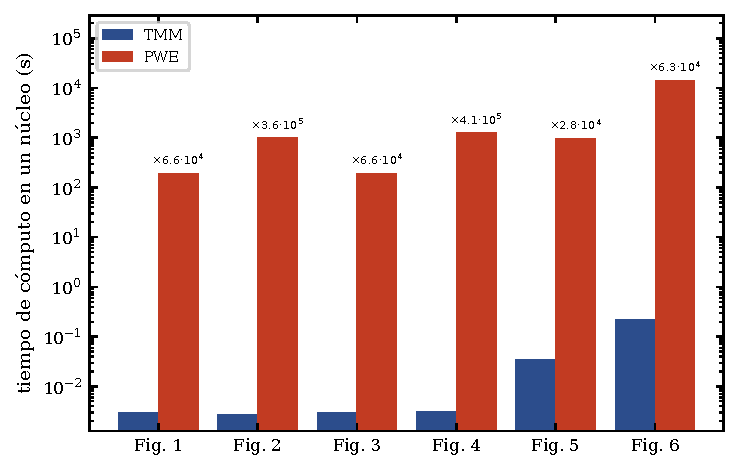
\includegraphics[width=0.62\linewidth]{comparison/timing/output/timing.pdf}
\caption{Tiempo en un núcleo de cada figura, con la razón PWE/TMM sobre cada par
de barras (escala logarítmica).}
\label{fig:tiempo-figuras}
\end{figure}

Con la TMM, las seis figuras del paper cuestan en total \EffFigTmmTotal{} en un
núcleo; con el PWE, unas \EffFigPweTotal. La razón por figura va de
$\EffFigRatioMin$ a $\EffFigRatioMax$
(Tabla~\ref{tab:tiempo-figuras}, Fig.~\ref{fig:tiempo-figuras}). En las Figs.~5--6
la razón es menor porque ahí la TMM también se llama frecuencia por frecuencia
dentro del localizador de bordes y paga la sobrecarga del intérprete. Ni siquiera
repartiendo el PWE en 16 procesos se cierra la brecha: las Figs.~1--4 tardaron
entre \EffFigWallMin{} y \EffFigWallMax~s de pared, frente a
\EffFigTmmMin--\EffFigTmmMax~ms de la TMM.

\subsection{Caso favorable al PWE: cristal no dispersivo}

El PWE tiene una ventaja estructural: en la forma $\omega(k)$, con materiales no
dispersivos, un solo problema de autovalores hermítico entrega \emph{todas} las
bandas en un $k$. Para verlo se calcularon 8 bandas en 41 valores de $k$ en el
cristal del libro ($\varepsilon_1=1$, $\varepsilon_2=9$). Por el lado de la TMM se
buscaron las raíces de $R(\omega)=\cos ka$ con el método de Brent
(Tabla~\ref{tab:libro-tiempo}). Aun en este caso, el más favorable para el PWE,
los dos métodos quedan en el mismo orden de tiempo (\EffBookPwe{} del PWE frente a
\EffBookTmm{} de la TMM), pero la TMM es exacta y el PWE tiene un error de
$\EffBookErr$. Y si se usa la TMM como es natural en 1D, es decir,
$k=\arccos R(\omega)$ sobre \EffBookGridPoints{} frecuencias, el diagrama de bandas
completo sale en \EffBookGrid. Con materiales de Drude
esta ventaja desaparece: la forma $\omega(k)$ se contamina con modos espurios
(Sec.~\ref{sec:contaminacion}), y la forma $k(\omega)$ requiere un problema de
autovalores por frecuencia, igual que la TMM requiere una evaluación.

\begin{table}[H]
\centering
\caption{Cristal no dispersivo del libro: tiempo en un núcleo para obtener las
mismas bandas.}
\label{tab:libro-tiempo}
\tabla{efficiency_book}
\end{table}

\subsection{¿Cuál método es más óptimo y por qué?}

\begin{table}[H]
\centering
\caption{Comparación de los dos métodos para superredes de Fibonacci 1D con
metamateriales de Drude (cifras de este anexo).}
\label{tab:decision}
\small
\renewcommand{\arraystretch}{1.3}
\begin{tabular}{>{\raggedright\arraybackslash}p{3.0cm}>{\raggedright\arraybackslash}p{5.6cm}>{\raggedright\arraybackslash}p{5.9cm}}
\toprule
Criterio & TMM & PWE ($k(\omega)$, regla inversa) \\
\midrule
Exactitud & Exacta; solo redondeo ($\sim\!10^{-15}$) & Truncamiento de Fourier:
$10^{-7}$--$10^{-2}$ según el contraste; error $\propto N^{-3}$ \\
Costo por frecuencia & $O(m)$ con recurrencia, $O(F_m)$ con producto;
\EffTmmRecMin--\EffTmmScalar~$\mu$s & $O(N^3)$ con $N=2hF_m+1$; de ms a decenas
de s \\
Crecimiento con $m$ & Casi constante (recurrencia) & $\approx\times\EffPweGrowth$
por cada orden de Fibonacci \\
Memoria & Una matriz $2\times2$ & $64N^2$~bytes: \EffMemEight{} ($m=8$),
\EffExtrapBMem{} ($m=\EffExtrapBM$) \\
Seis figuras del paper & \EffFigTmmTotal & $\approx$\EffFigPweTotal{}
($\times\EffFigRatioMin$--$\EffFigRatioMax$) \\
Dispersión de Drude & $\varepsilon(\omega)$, $\mu(\omega)$ se evalúan directamente &
Bien en $k(\omega)$; $\omega(k)$ produce modos espurios \\
Cerca de $\nu_m$ & Estable & Bandas espurias a $\lesssim10^{-6}$~GHz; exige validar
con $1.5N$ \\
Parámetros numéricos & Ninguno & $h$ (o $N$), regla de factorización, ventana de
selección del modo \\
Implementación & Unas decenas de líneas & Toeplitz, factorización de Li, QEP,
forma compañera, selección de $k$ \\
Información adicional & Campos a partir de las matrices & Coeficientes de Fourier
del modo; todas las bandas a un $k$ si no hay dispersión \\
Generalización & Solo medios estratificados (1D) & Cristales 2D y 3D \\
\bottomrule
\end{tabular}
\end{table}

\paragraph{Veredicto.} Para este problema, superredes de Fibonacci
unidimensionales con metamateriales de Drude, \textbf{la TMM es el método óptimo}.
Hay tres razones:
\begin{enumerate}
\item \textbf{Es exacta.} La matriz de cada capa es la solución analítica de la
ecuación de onda, así que el resultado solo tiene error de redondeo. No hay que
elegir $N$ ni hacer estudios de convergencia, y sus bandas sirven de referencia
para medir el error del PWE.
\item \textbf{Es órdenes de magnitud más barata, y la diferencia crece con $m$.}
Su costo es $O(m)$ (o $O(F_m)$), frente a $O(N^3)\sim\varphi^{3m}$ del PWE. En
tiempo medido, eso son microsegundos frente a segundos por frecuencia, y
\EffFigTmmTotal{} frente a \EffFigPweTotal{} para las seis figuras. Con
$m\ge\EffExtrapAM$ el PWE deja de ser
práctico por tiempo y por memoria, mientras que la TMM sigue en
microsegundos.
\item \textbf{Es robusta donde está la física del paper.} Las subbandas de
plasmón-polaritón viven a $10^{-4}$--$10^{-2}$~GHz de $\nu_m$, donde $\mu_B\to0$.
La TMM es estable ahí, mientras que el PWE necesita una validación que duplica su
costo y aun así pierde validez a menos de $\sim10^{-6}$~GHz del polo.
\end{enumerate}

\paragraph{Para qué sirve entonces el PWE.} Su valor no está en la velocidad, sino
en otras tres cosas:
\begin{itemize}
\item Es una \emph{verificación independiente}: formulado en el espacio
recíproco, reproduce las mismas bandas, conteos y bordes, lo que descarta errores
sistemáticos de la TMM.
\item Entrega \emph{todas las bandas a un $k$} en cristales no dispersivos.
\item Es el método que se \emph{generaliza a cristales 2D y 3D}, donde no existe
una matriz de transferencia $2\times2$ (\code{PWE\_2D.m} del libro).
\end{itemize}
En 1D conviene usar la TMM para producir resultados y el PWE para validarlos. En
2D o 3D la elección se invierte.

%=====================================================================
\section{Conclusiones: los dos métodos implementados}
\label{sec:conclusiones}
%=====================================================================

\subsection*{Los resultados son los mismos}

Los dos métodos parten de formulaciones completamente distintas: la TMM multiplica
matrices en el espacio real y el PWE resuelve un problema de autovalores en el
espacio recíproco. Aun así, dan la misma semitraza, las mismas bandas y los mismos
gaps en las seis figuras del paper. La clasificación banda/gap coincide en más del
99.9\% de las frecuencias, el número de subbandas de plasmón-polaritón sigue la
regla $F_{m-2}$ con los dos métodos y los bordes de subbanda coinciden con errores
relativos de ancho menores que $10^{-5}$. Como los dos métodos no comparten ninguna
parte del cálculo salvo los parámetros físicos, este acuerdo valida la
reimplementación del paper con mucha más fuerza que cualquiera de los dos por
separado.

\subsection*{Matriz de transferencia (TMM)}

\begin{itemize}
\item \textbf{Fortalezas.} Es exacta para medios estratificados: la matriz de cada
capa es la solución analítica de la ecuación de onda y el único error es el de
redondeo ($\sim\!\EffWpTmmErr$). Admite la dispersión de Drude sin ningún
tratamiento especial, porque $\varepsilon(\omega)$ y $\mu(\omega)$ se evalúan en
cada frecuencia. Con la recurrencia de semitrazas su costo es $O(m)$
(\EffTmmRecMin--\EffTmmScalar~$\mu$s por frecuencia hasta
$m=\EffTmmMaxM$), usa la memoria de una matriz $2\times2$, no tiene parámetros
numéricos que ajustar y es estable junto a $\nu_m$, donde vive la física de los
plasmón-polaritones.
\item \textbf{Límites.} Solo sirve para medios estratificados (1D). Da $R(\omega)$
frecuencia por frecuencia, así que las bandas $\omega(k)$ se obtienen buscando
raíces o evaluando sobre una malla, y en los gaps profundos $|R|$ crece
exponencialmente con $m$, lo que obliga a comparar con errores relativos.
\end{itemize}

\subsection*{Expansión en ondas planas (PWE)}

\begin{itemize}
\item \textbf{Fortalezas.} Es una verificación independiente de la TMM. En la
forma $\omega(k)$ con materiales no dispersivos entrega todas las bandas de un $k$
con un solo problema de autovalores hermítico, y es el método que se generaliza a
cristales 2D y 3D, donde no existe una matriz de transferencia $2\times2$. La forma
$k(\omega)$ con la regla inversa de Li maneja correctamente la dispersión de Drude
y el alto contraste.
\item \textbf{Límites.} Es aproximado: el truncamiento de Fourier de un perfil
discontinuo deja un error que baja solo algebraicamente
($\propto N^{-\EffWpErrExp}$) y que crece donde el contraste es alto
($\nu\lesssim0.5$~GHz) o junto al polo de $1/\mu_B$. Cuesta $O(N^3)$ con
$N=2hF_m+1\propto\varphi^m$, necesita $64N^2$~bytes de memoria y depende de
parámetros numéricos ($h$, regla de factorización, selección del modo). En la
forma $\omega(k)$ con Drude aparecen modos espurios, y a menos de
$\sim\!10^{-6}$~GHz de $\nu_m$ produce bandas espurias que hay que descartar
validando con $1.5N$ ondas planas.
\end{itemize}

\subsection*{Tiempo y método óptimo}

Medidos en las mismas condiciones (un núcleo, un hilo de BLAS), la TMM reproduce
las seis figuras del paper en \EffFigTmmTotal{} y el PWE en unas \EffFigPweTotal,
entre $\EffFigRatioMin$ y $\EffFigRatioMax$ veces más por figura. La brecha crece
con el orden de Fibonacci: el PWE pasa de \EffPweFirst{} ($m=\EffPweFirstM$) a
\EffPweLast{} ($m=\EffPweLastM$) por frecuencia y para $m=\EffExtrapBM$ tardaría
unas \EffExtrapB{} por frecuencia con \EffExtrapBMem{} de memoria, mientras que la
TMM sigue en fracciones de microsegundo. Para una misma precisión la diferencia es
aún mayor: el mejor resultado del PWE ($\EffWpBestErr$) cuesta \EffWpBestTime{}
por frecuencia, y la TMM llega al redondeo de la máquina en microsegundos. Ni
siquiera en el caso más favorable al PWE, el cristal no dispersivo del libro, la
TMM queda por detrás.

Por lo tanto, \textbf{para las superredes de Fibonacci unidimensionales con
metamateriales de Drude del paper, la TMM es el método óptimo}: es exacta, es
órdenes de magnitud más rápida, su ventaja crece con $m$ y es robusta cerca de
$\nu_m$.

\subsection*{Cuándo usar cada uno}

En 1D conviene producir los resultados con la TMM y usar el PWE para validarlos de
forma independiente, que es exactamente el papel que cumplió en este trabajo. El
PWE recupera su lugar en cristales fotónicos 2D y 3D, donde la TMM no se puede
aplicar y la expansión en ondas planas es la herramienta estándar; la
implementación 1D de este proyecto, con la regla inversa y la forma $k(\omega)$
para materiales dispersivos, es la base para ese paso.

\section*{Reproducibilidad}
\begin{lstlisting}
python scripts/tmm/run_all.py          # resultados TMM   -> results/tmm/
python scripts/pwe/run_all.py          # resultados PWE   -> results/pwe/
python scripts/comparison/run_all.py   # comparacion      -> results/comparison/
python scripts/comparison/efficiency.py --plot-only   # redibuja tiempos sin medir
make pwe-docs                          # compila el paper del PWE y este anexo
make verify                            # aceptacion, tablas, figuras y PDF
make all                               # pruebas, resultados, documentos y verificacion
\end{lstlisting}

\end{document}
